\section{预设性能控制(Prescribed Performance Control)}\label{4Fref}

考虑下述标量系统
\begin{equation*}
    \dot{x} = u + \varphi(x)\theta
\end{equation*}
其中$x$为状态,$u$为控制输入,$\varphi$是已知的连续函数,$\theta$为未知常数。

我们的{\bf 控制目标}是:
\begin{itemize}[leftmargin=1em]
    \item 闭环系统的所有信号都是有界的;
    \item 状态$x$能跟踪期望状态轨线$x_d(t)$;
    \item 误差$e(t)=x(t)-x_d(t)$达成指定的瞬态和稳态性能指标
\end{itemize}

前两点目标是我们一直探讨的话题。特殊的是第三点目标。我们采取下面这样一类函数来描述这个目标。
\begin{definition}[性能函数(performance function)]\label{performance_func}
   称光滑的函数$\rho(t):\mathbf{R}_+\to\mathbf{R}_+$
   为{\bf 性能函数},若其满足
   \begin{itemize}[leftmargin=1em]
    \item $\rho(t):\mathbf{R}_+\to\mathbf{R}_+$为正且递减;
    \item $\lim\limits_{t\to\infty}\rho(t)=\rho_\infty>0$。
\end{itemize}
\end{definition}
\begin{example}[性能函数]
   $\rho(t)=(\rho_0-\rho_{\infty})\mathrm{e}^{-\lambda t}+\rho_\infty$($\lambda,\rho_0,\rho_{\infty}>0$)是一个性能函数。其图形如下:
   \begin{center}
       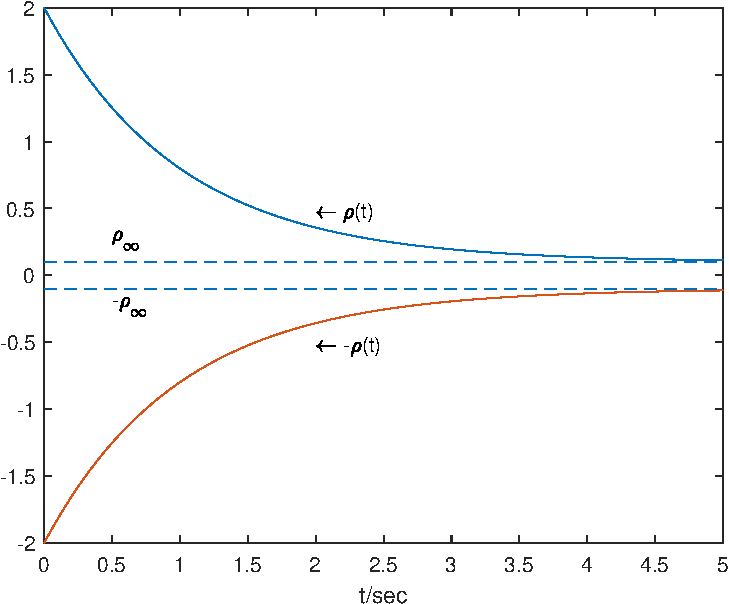
\includegraphics[scale=0.5]{figure/adaptive/p.pdf}
       \captionsetup{hypcap=false}
       \captionof{figure}{上述性能函数的图形($\lambda=1,\rho_0=2,\rho_{\infty}=0.1$)}
   \end{center}
\end{example}
我们欲使$|e(t)|<\rho(t)$,那么通过指定合适的$\rho(t)$,即可限制误差的稳态和瞬态特性。

为了应用之前手段(分析信号的有界性)来分析上述问题,我们引入以下{\bf 误差转换(error transformation)},将上述有约束的跟踪误差变为等价的无约束问题。

具体而言,我们定义\[e(t)=\rho(t)T(\zeta)\]
其中$\zeta$是变换后的无约束误差,$T(\zeta)$是光滑的函数,并具有如下性质:
\begin{itemize}[leftmargin=1em]
    \item $T(\zeta)$严格单调递增;
    \item $\lim\limits_{\zeta\to-\infty}T(\zeta)=-1$,$\lim\limits_{\zeta\to\infty}T(\zeta)=1$。
\end{itemize}
则有
\[\zeta = T^{-1}\left(\frac{e(t)}{\rho(t)}\right)\]
$\frac{e(t)}{\rho(t)}\to -1$时,$\zeta\to-\infty$;$\frac{e(t)}{\rho(t)}\to 1$时,$\zeta\to\infty$。
我们发现,如果$\zeta$有界,那么$-1<\frac{e(t)}{\rho(t)}<1$,这样,分析$\zeta$的有界性就等价于分析误差满足的约束。

\begin{example}
    以下两个$T^{-1}$都是可行的:
    \[\zeta = \tan\left(\frac{\pi}{2}\frac{e(t)}{\rho(t)}\right),\zeta = \ln\left(\frac{e(t)+\rho(t)}{\rho(t)-e(t)}\right)\]
\end{example}

接下来对$\zeta$的动力学进行分析:
\begin{align*}
    \dot{\zeta} &= \frac{\partial T^{-1}}{\partial \left(\frac{e(t)}{\rho(t)}\right)}
    \frac{\diff}{\diff t}\left(\frac{e(t)}{\rho(t)}\right)
\end{align*}
易知第一个因子为正定(因$T^{-1}$随$\left(\frac{e(t)}{\rho(t)}\right)$单调递增),记其为$R$。
则上式等于
\begin{align*}
    \dot{\zeta} &= R
    \frac{\diff}{\diff t}\left(\frac{e(t)}{\rho(t)}\right)\\
    &=R\frac{\dot{e}(t)\rho(t)-e(t)\dot{\rho}(t)}{\rho^2(t)}\\
    &=\frac{R}{\rho(t)}(u+\varphi(x)\theta-\dot{x}_d(t))-\frac{Re(t)\dot{\rho}(t)}{\rho^2(t)}
\end{align*}
可选取\[u=-\varphi(x)\hat{\theta}+\frac{\dot{\rho}(t)}{\rho(t)}e(t)+\dot{x}_d(t)+\frac{\rho(t)}{R}u_0\]
以消去第二项与括号中第三项,得到
\[\dot{\zeta} = u_0-\frac{R}{\rho(t)}\varphi(x)\tilde{\theta}\]
其中$\tilde{\theta}\triangleq \hat{\theta}-\theta$。
于是进一步选取$u_0=-k\zeta,k>0$,有
\[\dot{\zeta} = -k\zeta-\frac{R}{\rho(t)}\varphi(x)\tilde{\theta}\]
考虑如下候选Lyapunov函数
\[V=\frac{1}{2}\zeta^2+\frac{1}{2\gamma}\tilde{\theta}^2,\gamma>0\]
求其导数得\begin{align*}
    \dot{V}&=\zeta\left(-k\zeta-\frac{R}{\rho(t)}\varphi(x)\tilde{\theta}\right)+\frac{1}{\gamma}\tilde{\theta}\dot{\hat{\theta}}\\
    &=-k\zeta^2+\frac{1}{\gamma}\tilde{\theta}\left(\dot{\hat{\theta}}-\gamma \frac{R}{\rho(t)}\varphi(x)\zeta\right)
\end{align*}
设计\[\dot{\hat{\theta}}=\gamma \frac{R}{\rho(t)}\varphi(x)\zeta\]
则$\dot{V}=-k\zeta^2\le 0$,类似 \ref{4Bref} 节各例可分析$\zeta$有界性。进而$|e(t)|<\rho(t)$,达成了我们的目标。

进一步地,如果我们超调量有要求,即要求$e(t)$穿过横轴时的下冲/上冲(具体由$e(0)$的正负而定,即$e(0)$为正时限制下冲,$e(0)$为负时限制上冲)要小,如何考虑该问题?
我们发现,如指定超调小于$\delta\rho(0)$($0\le\delta\le 1$。此为常值,故假定是可行的),则要求$-\delta\rho(t)<e(t)<\rho(t)$(若$e(0)>0$)或$-\rho(t)<e(t)<\delta\rho(t)$(若$e(0)<0$)即可。

类似本节前述思路进行误差转换。定义\[e(t)=\rho(t)T(\zeta)\]
其中$\zeta$是变换后的无约束误差,$T(\zeta)$仍为光滑且单调递增的函数,并且:
\begin{itemize}[leftmargin=1em]
    \item 若$e(0)>0$,则$\lim\limits_{\zeta\to-\infty}T(\zeta)=-\delta$,$\lim\limits_{\zeta\to\infty}T(\zeta)=1$;
    \item 若$e(0)<0$,则$\lim\limits_{\zeta\to-\infty}T(\zeta)=-1$,$\lim\limits_{\zeta\to\infty}T(\zeta)=\delta$。
\end{itemize}

\begin{example}
    以下$T$是可行的:
    \[T(\zeta) = \begin{cases}
        \frac{\mathrm{e}^\zeta-\delta \mathrm{e}^{-\zeta}}{\mathrm{e}^\zeta+ \mathrm{e}^{-\zeta}}&e(0)>0\\
        \frac{\delta\mathrm{e}^\zeta- \mathrm{e}^{-\zeta}}{\mathrm{e}^\zeta+ \mathrm{e}^{-\zeta}}&e(0)<0
    \end{cases}\]
\end{example}
之后类似本节前述思路进行控制器设计,使$\zeta$有界即可。

更一般地,我们可以将上下界取为不同的函数,即
\[\rho_1(t)<e(t)<\rho_2(t)\]
其中$\rho_1(t),\rho_2(t)$都是定义如 \ref{performance_func} 的性能函数。

进行误差转换。定义\[e(t)=T(\zeta,\rho_1(t),\rho_2(t))\]
其中$\zeta$是变换后的无约束误差。
则\[\zeta = T^{-1}(e(t),\rho_1(t),\rho_2(t))\]
因此,我们要求\[\lim\limits_{\zeta\to-\infty}T(\zeta,\rho_1(t),\rho_2(t))=\rho_1(t),\lim\limits_{\zeta\to\infty}T(\zeta,\rho_1(t),\rho_2(t))=\rho_2(t)\]
\begin{example}
    以下$T^{-1}$是可行的:
    \[\zeta = \tan\left(\frac{\pi}{2}\frac{2e(t)-\rho_1(t)-\rho_2(t)}{\rho_2(t)-\rho_1(t)}\right)\]
\end{example}

之后类似本节前述思路进行控制器设计,使$\zeta$有界即可。